%%%% outstanding mysteries %%%%%
% error bar on 0-1 peak height (mention in text)
% can I cite someone as to why \Delta_ST changes with field
% dS or \partial S?
% why does \partial S/ \partial N

\documentclass[preprint,showpacs,preprintnumbers,amsmath,amssymb,pra,aps,superscriptaddress]{revtex4-1}

\usepackage{graphicx}
\usepackage{amsmath}
\usepackage{siunitx}
\usepackage{hyperref}

\begin{document}

\title{Direct Entropy Measurement in a Mesoscopic Quantum System}
\author{Nikolaus Hartman}
\email{nik.hartman@gmail.com}
\thanks{The raw data and Python code used for the figures and analysis can be found at \url{https://github.com/nikhartman/spin_entropy}}
\affiliation{University of British Columbia, Vancouver, BC, Canada}
\author{Saeed Fallahi}
\affiliation{Purdue University, Lafayette, IN, USA}
\author{Geoffrey C. Gardner}
\affiliation{Purdue University, Lafayette, IN, USA}
\author{Christian Olsen}
\affiliation{University of British Columbia, Vancouver, BC, Canada}
\author{Silvia Folk}
\affiliation{University of British Columbia, Vancouver, BC, Canada}
\author{Mohammad Samani}
\altaffiliation{The Hospital for Sick Children, Toronto, ON, Canada}
\altaffiliation{Fields Institute for Research in Mathematical Sciences, Toronto, ON, Canada}
\affiliation{University of British Columbia, Vancouver, BC, Canada}
\author{Michael Manfra}
\affiliation{Purdue University, Lafayette, IN, USA}
\author{Joshua Folk}
\affiliation{University of British Columbia, Vancouver, BC, Canada}
\date{\today}

\begin{abstract}

%Measuring the entropy of an electronic state is a powerful tool for identifying its underlying microscopic character.  Such measurements are typically based on bulk properties, such as heat capacity, that are straightforward to observe in macroscopic samples but exceedingly difficult to access in mesoscopic systems that may consist of just a few electrons. Taking advantage of a well-known Maxwell relation, we realize a protocol for entropy-to-charge conversation in a gate-defined GaAs quantum dot that enables an entropy measurement of the first three quantum states in to the dot. The entropy of a single spin ($k_B \ln{2}$) is measured within 8\% accuracy, as is the entropy arising at the magnetic field-driven singlet-triplet crossing for two electrons.

\end{abstract}

\maketitle

%%%%%%% intro material %%%%%%%%%
The thermodynamic properties of electronic systems can offer important insights into the nature of their ground states, and probe exotic quasiparticles that may emerge due to interactions or non-trivial topology.  Systems that are difficult to clearly identify through standard conductance measurements may be studied more in depth if a thermodynamic measurement can be made. For example, the purported non-Abelian exchange statistics of Moore-Read quasiparticles in the $\nu = \frac{5}{2}$ fractional quantum Hall state, or of Majorana quasiparticles in a topological superconductor, are exceedingly difficult to identify from conductance signatures. However, an entropy measurement could clearly distinguish Abelian from non-Abelian quasiparticles \cite{Cooper2009, Smirnov2015}.  Similarly, the two-channel Kondo state that is believed to arise in carefully tuned GaAs devices has so far been identified through a particular temperature dependence in the device conductance \cite{Potok2007}. A more direct test for the two-channel Kondo state would be a confirmation of its entropy ($\frac{1}{2} k_B \ln{2}$), that should remain down to arbitrarily low temperatures \cite{Alkurtass2016}.

%%% figure 1 %%%
\begin{figure}[!]
        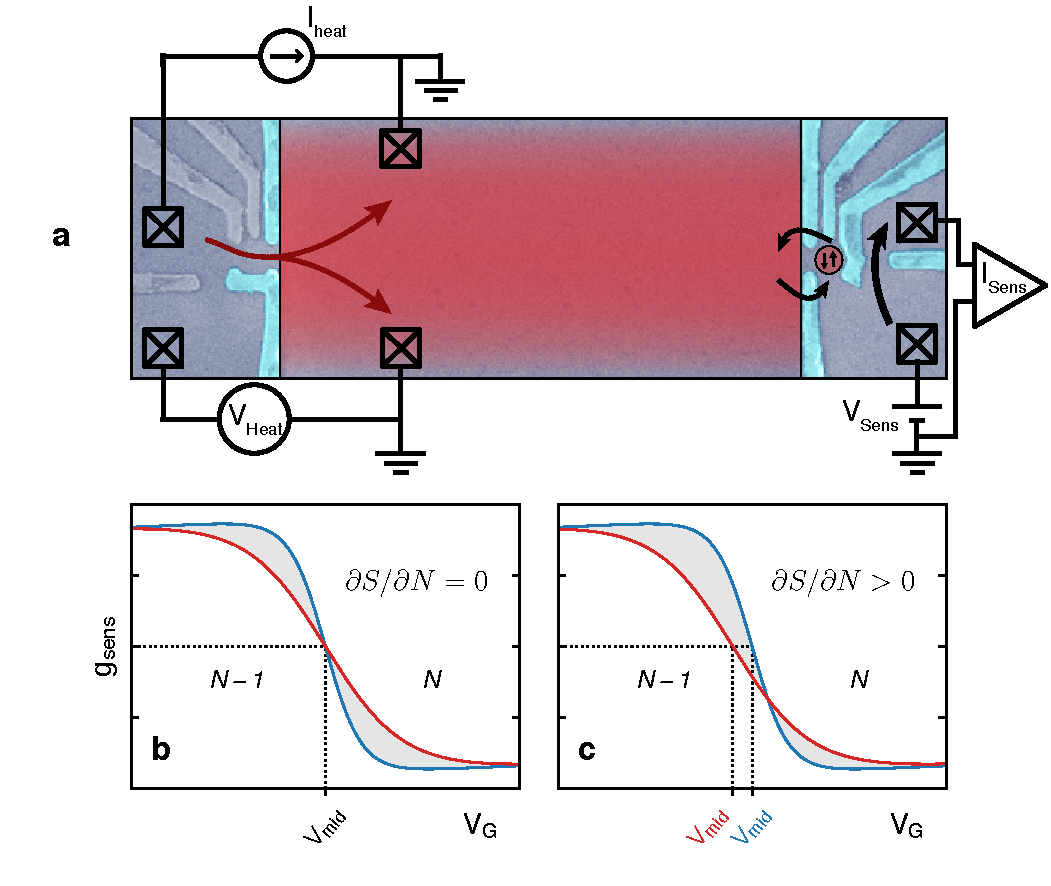
\includegraphics[width=1.0\columnwidth]{../figures/figure_1_no-annotation.pdf}
        \caption{\label{fig:fig1}(a) Scanning electron micrograph of a device similar to the one measured, showing electrostatic gates (blue) used to define a circuit in the 2D electron gas. Grey gates are unused (grounded). Squares show the locations of ohmic contacts to the 2DEG. An electron reservoir is formed between the parallel gates running vertically down the image, with a 200nm diameter quantum dot coupled to the right side. The channel can be heated by driving current through the quantum point contact on the left. Electrons tunneling between the reservoir and dot are measured with a capacitively-coupled charge sensor. (b)  Charge sensor signal showing a single transition from $N \rightarrow N+1$ electrons at two temperatures ($T_{Red} > T_{Blue}$). (c) Change in the charge sensor signal with respect to temperature. The asymmetry in peak height arises from a shift in $V_0$ that would arise from a change in entropy between the $N$ and $N+1$ electron states. In the case of $dS=0$, $dg_{sens}$ is anti-symmetric about $V_0$.}
\end{figure}

Entropy can be probed effectively in 3D macroscopic samples via measurements of heat capacity, but the heat capacities of single electrons or quasiparticles are much too small to measure directly; even the 2D sheet of quasiparticles in $\nu = \frac{5}{2}$ fractional quantum Hall samples has a heat capacity that vanishes in comparison to that of the host crystal.  Rather than attempt to resolve such infinitesimal signals, the problem can be avoided by converting a change in entropy to changes in charge--a quantity that is easily detected at the single particle level.  Our approach is analogous to the milestone of spin-to-charge conversion, first demonstrated in GaAs quantum dots in 2004, by which undetectably-small magnetic moments of a single spin were transformed into the presence or absence of an electron charge \cite{Elzerman2004, Ono2004}.

In order to accomplish this entropy to charge conversion, we make use of the Maxwell relation
%
\begin{align}
\label{eqn:max}
        \left(\frac{\partial \mu}{\partial T}\right)_{p,N} &= -\left(\frac{\partial S}{\partial N}\right)_{p,T}
\end{align}
%
that connects changes in entropy, $S$, (as well as particle number, $N$, and temperature, $T$) to changes in the chemical potential, $\mu$, a quantity that is simple to measure and control. The fixed pressure condition of Eq.~\ref{eqn:max} is effectively met by working well below the Fermi temperature, $T_F \sim$\SI{5}{\kelvin}, where the pressure is simply the degeneracy pressure \cite{Landau1969}.

This Maxwell relation forms the basis of two exciting proposals to measure the entropy derivative, $\frac{\partial S}{\partial N}$, of the $\nu = \frac{5}{2}$ state by detecting changes in the quasiparticle chemical potential with temperature, though these have not yet been realized in experiment \cite{Cooper2009,Ben-Shach2013}.  Our work builds on these proposals to measure the entropy of the few-electron ground states of a quantum dot. Unlike the $\nu = \frac{5}{2}$ quasiparticles described in the theoretical work, the few-electron quantum dot states studied here have an entropy that is well-understood from the spin degree of freedom \cite{Tarucha1996, Ciorga2000, Duncan2000, Lindemann2002, Potok2003, Hofmann2016}. Our experiment demonstrates a direct entropy measurement on a few-particle system; in the future, the method can be easily extended as a probe into the nature of more exotic systems, such as topologically non-trivial Majorana and other non-Abelian states.

The mesoscopic circuit shown in Fig.~\ref{fig:fig1}a uses electrostatic gates to realize an electron reservoir (central region; hereafter ``reservoir") in thermal and electrochemical equilibrium with a few-electron quantum dot (``dot") coupled to its right side.  The occupation of the dot is measured using an adjacent quantum point contact (``charge sensor")\cite{Staring2007, Frolov2009, Thierschmann2015}.  The $N+1^{\rm st}$ electron is added to an $N$ electron dot when the chemical potential, $\mu_{N+1}$, tuned by the gate voltage, $V_G$, drops below the Fermi level of the reservoir, $E_F$.  

Figure 1b illustrates a such a transition---a step in the charge sensor conductance as a function of $V_G$---thermally broadened by the reservoir temperature, $T_{res}$.  The gate voltage corresponding to midpoint of the transition, $V_0$, marks the chemical potential where the probabilities of finding $N$ or $N+1$ electrons on the dot are equal.
%In practice, the shift in $V_0$ with temperature is measured by oscillating $T_{res}$ and monitoring any resulting changes in $g_{sens}$ with a lockin amplifier.  If the transition is broadened but not shifted due to heating ($dS=0$), an antisymmetric lineshape is expected from this lockin measurement.  If the transition is not only broadened but also shifted ($dS,d\mu\neq0$), the change in $g_{sens}$ due to heating will asymmetric, as shown in Fig.~\ref{fig:fig1}c, thus offering a clearly distinguishable signature of entropy for this single charge measurement.
According to Eq.~\ref{eqn:max}, the chemical potential and therefore $V_0$ shifts with temperature by an amount that is proportional to the entropy difference between the $N$ to $N+1$ ground states ($\delta S_{N\rightarrow N+1}$ for $\delta N=1$).  This shift is the quantity probed directly in the experiment described below; from these measurements the entropy of the first three energy levels in the quantum dot are built up, one by one.  Before turning to the experiment in detail, it is helpful to consider the same physics from an alternate point of view.
  
The relation between entropy and a temperature-induced shift in $\mu_{N+1}$ (with respect to $E_F$) can also be understood in the language of detailed balance.   Generically, the $N+1^{\rm st}$ electron tunnels back and forth between an $N$-electron dot and a reservoir as long as there are available states in both dot and reservoir, that is, as long as $\mu_{N+1}$ is within thermal broadening of $E_F$.  The tunnel rates into and out of the dot, $\Gamma_{in}=\Gamma_{N\rightarrow N+1}$ and $\Gamma_{out}=\Gamma_{N+1\rightarrow N}$, depend on degeneracy of the $N$ and $N+1$ ground states.  Consider the filling of the first electron state at zero magnetic field, a state with a single, unpaired spin-$\frac{1}{2}$ and therefore a degeneracy of 2. An electron tunneling in has both spin-up and -down states available.  Tunneling out, the electron (whether spin-up or -down) must tunnel into reservoir states with the same spin, that is, only half of the reservoir states are available. As a result, $\Gamma_{in} = 2\Gamma_{out}$ when $\mu_{N+1}=E_F$. Extending this logic to a general case gives the result derived from detailed balance \cite{Gustavsson2009}, 
%
\begin{align}
	\Gamma_{in} &=  g_{N+1} \Gamma f(E_F - \mu_{N+1}) \label{eqn:rates}\\
	\Gamma_{out} &= g_{N} \Gamma [1 - f(E_F - \mu_{N+1})] \nonumber
\end{align}
%
where $\Gamma$ is a coupling constant, $f$ is the Fermi function, and $g_{N(N+1)}$ is the degeneracy of the $N(N+1)$ electron state.

The midpoint of the transition between the $N$ and $N+1$ electron states ($V_0$), as measured by the charge sensor, occurs when the dot is occupied half the time, that is, when $\Gamma_{in} = \Gamma_{out}$. From Eq.~\ref{eqn:rates}, $\Gamma_{in} = \Gamma_{out}$ corresponds to $\mu_{N+1} = E_F$ when $g_{N}=g_{N+1}$, but shifts away when $g_{N}\neq g_{N+1}$ by an amount that depends on the broadening of the Fermi function, and therefore on $T$.   A measurement of how $V_0$ shifts with T allows the ratio $g_{N+1}/g_{N}$ to be determined, which itself is related to $dS_{N\rightarrow N+1}$ through the Boltzmann entropy formula, $S_{N}=k_{B} \ln{g_N}$.  The relationship between degeneracies and tunnel rates was recently explored in a time-resolved measurement \cite{Hofmann2016}.  The thermal technique presented here extends the measurement of entropy (degeneracy) to a wider set of applications, where the tunneling process may not be convenient or even possible to observe in real-time.

%%% fab/measurement details %%%

%%%%%%%%%%%%%%%%%%%%%%%

%%% figure 2 %%%
\begin{figure}[!]
        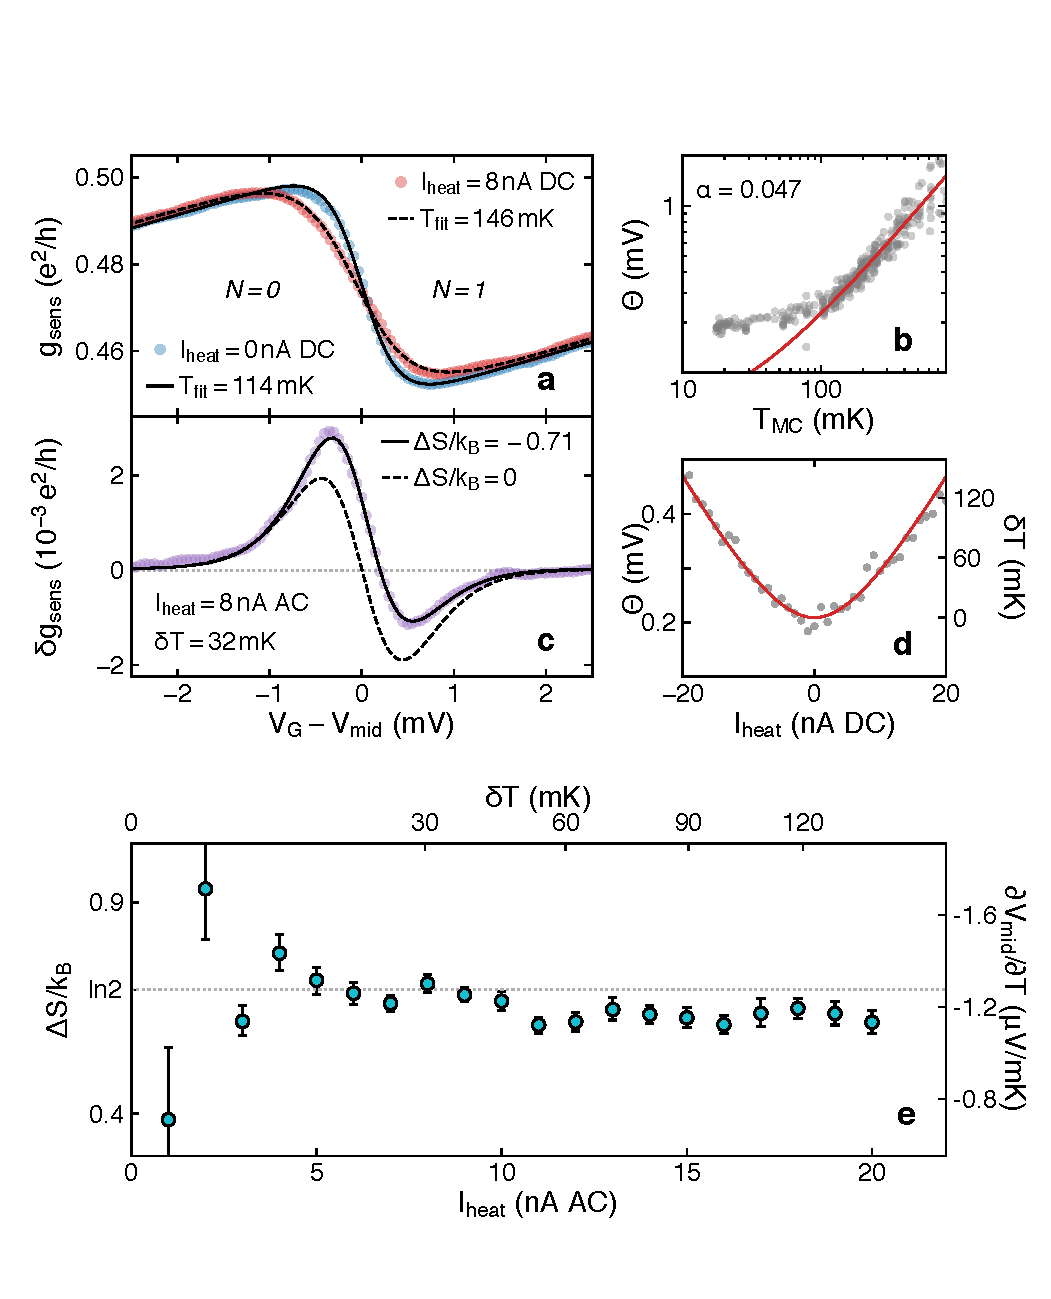
\includegraphics[width=1.0\columnwidth]{../figures/figure_2.pdf}
        \caption{\label{fig:fig2}(a) Charge sensor data for $N=0 \rightarrow 1$ at 100 and 160mK. Temperature is set by DC current through the QPC heater. (b) Lockin measurement of $dg_{sens}$ with $dT \sim 60mK$. Fits to $dg_{sens}$ are shown with $\delta$ as a free parameter (solid) and $\delta=0$ (dashed) (c) Transition width, $\Theta$, as a function of mixing chamber temperature. The highlighted, linear region is where the tunnel rates are determined only by temperature broadening. The lever arm $\alpha$ is calculated by fitting a straight line to this region. (d) $\Theta$ as a function of DC current through the QPC heater. Linear fit is used to convert between $I_{heat}$ and $dT$, with $R_{QPC} = $ \SI{20}{\kilo\ohm} (e) Change in entropy as a function of AC current through the QPC heater. Top axis shows corresponding $dT$. Right axis shows shift in $V_0$ per unit temperature.}
\end{figure}

%%% device setup %%%
We now turn to the details of the experiment.  The quantum dot (Fig.~1a) was tuned such that the source was weakly tunnel coupled to the reservoir with the drain closed. The conductance of the charge sensor,  $g_{sens}$, was measured in a DC voltage biased configuration, and tuned to $g_{sens}{\sim}e^2/h$ where it was maximally sensitive to charge on the dot.  The reservoir temperature could be rapidly controlled (up to at least  \SI{100}{\hertz}) by by Joule heating through the QPC on the left side (Fig.~1a), which was fixed at \SI{20}{\kilo\ohm} and biased with an AC or DC current source.

%%% figs 2a and b %%%
The addition of the first electron to the dot was marked by a decrease in $g_{sens}$ that is well fit by the expected form for a thermally-broadened transition (Fig.~\ref{fig:fig2}a):
%by tuning $V_G$, at two different temperatures. The higher temperature transition curve is noticeably broadened by the increased temperature. Assuming the source barrier is sufficiently large, $\Gamma_{in/out}$ are broadened only by the temperature of the reservoir and the conductance takes the form,

%
\begin{align}
\label{eqn:g}
        g_{sens}(V,\Theta) &= G_0 \tanh\left(\frac{V-V_0(\Theta)}{2\Theta}\right)  \\
                        &\quad + G_1\left[V-V_0(\Theta)\right] + G_2 \nonumber
\end{align}
%
where $G_0$ quantifies the sensor sensitivity, $\Theta = \frac{k_B T}{\alpha e}$ is the thermal broadening expressed in units of gate voltage, $\alpha$ is the lever arm that converts $V_G$ to quantum dot potentials, and $G_1$ is determined by the cross capacitance between the sensor and the plunger gate. The dependence of $V_0$ on $\Theta$ captures any shift in $\mu$ due to a change in entropy across the transition.
%Fits to Eq.~\ref{eqn:g} are seen, in addition to the sensor data, in Fig.~\ref{fig:fig2}a.

The transition width, $\Theta$, extracted from fits to Eq.~\ref{eqn:g} follows the mixing chamber temperature, $T_{MC}$, down to below 100 mK (Fig.~\ref{fig:fig2}b)
%; $\alpha$ can be calculated based on this linear trend in the high temperature limit.
The assumption of thermally broadened transitions greatly simplifies the data analysis, so $T_{MC}$ is fixed at \SI{100}{\milli\kelvin} for most of this work, with Joule heating giving reservoir temperatures up to \SI{160}{\milli\kelvin}, still cold enough that no orbital levels above the ground state were excited.
%Fitting high temperature data in Fig.~\ref{fig:fig2} to the definition of $\Theta$ (with $T=T_{MC}$) yields $\alpha$, making it possible to convert from $V_G$ to $\mu$.

%%% figs 2c and d%%%
The data in Fig.~\ref{fig:fig2}c, and corresponding fits, offer an example of how $dS_{0\rightarrow 1}$ was measured across the $0 \rightarrow 1$ transition. A comparison of the 100 and 160 mK data in Fig.~\ref{fig:fig2}a shows that $g_{sens}$ drops as the temperature rises before the midpoint of the transition ($V_G-V_0<0$), whereas the conductance is higher in the warmer curve for $V_G-V_0>0$.   Oscillating the reservoir temperature by $dT_{res}$ using an AC current, $I^{AC}_{Heat}$, through the heater QPC, while locking in to resultant oscillating $dg_{sens}$ yields the characteristic peak-dip structure seen in Fig.~\ref{fig:fig2}c.  The expected lineshape of such a curve is given by the derivative of Eq. \ref{eqn:g} with respect to temperature, expressed as $dg_{sens}$ due to a temperature change $dT$:

%If $V_0$ did not change with $T_{res}$, one would expect a perfectly antisymmetric lineshape.  When $V_0$ changes with  $T_{res}$, on the other hand, as expected when there is an entropy change between the two charge states, the lineshape is not perfectly antisymmetric: this is the case shown in Fig.~\ref{fig:fig2}c. 

%
\begin{align}
\label{eqn:dg}
        dg_{sens}(V_G, \Theta) &\propto dT \left[ \frac{V_G-V_0}{2\Theta} +\delta \right]\times \\
        				      &\quad\cosh^{-2}\left(\frac{V_G-V_0}{2\Theta}\right) \nonumber
\end{align}
%
where $\delta=\frac{\partial V_0}{\partial \Theta}$. Using the lever arm to convert $V_0$ to chemical potential, one sees that the parameter $\delta$ is simply the change in entropy scaled by Boltzmann's constant:
%
\begin{align}
\label{eqn:delta}
        \delta &= \frac{\partial V_0}{\partial \Theta} = 
        \frac{1}{k_B} \frac{\partial \mu}{\partial T} = 
        -\frac{1}{k_B} \partial S_{N\rightarrow N+1}
\end{align}
%

From Eq.~\ref{eqn:dg}, $dg_{sens}(V_G)$ would perfectly antisymmetric around $V_0$ if $\partial S_{N\rightarrow N+1}$ were zero.  Fits to the data in Fig.~\ref{fig:fig2}c illustrate clearly that $\partial S_{0\rightarrow 1}=0$ is inconsistent with the data;  the best fit is found for $\partial S_{0\rightarrow 1}=0.71\times k_B$.  Indeed, this is what would be expected for the $0 \rightarrow 1$ electron transition at zero magnetic field: $S_0$ for the empty state should be $k_B \ln{1}=0$ whereas for the spin degenerate 1-electron state one expects $S_1=k_B\ln{2}$, giving $dS_{0\rightarrow 1}\equiv S_1 = S_0 =k_B\ln{2}$.%%% fig 2e %%%
Note that $\delta$ is a fit parameter that is independent of $dT$ and $\alpha$. Fig.~\ref{fig:fig2}e shows that $dS$,  determined from fits to data analogous to Fig.~\ref{fig:fig2}c, remains constant over a range of $dT$ ($I^{AC}_{Heat}$).  Although the extracted $\delta$ can be converted to gate-voltage-per-temperature units using a value for $\alpha$ measured separately (right axis of Fig.~\ref{fig:fig2}e), the entropy itself, $dS$, is determined directly from the fit to $g_{sens}$ without any additional calibration.
%The vertical scale on the right side of Fig. \ref{fig:fig2}e converts $\delta$ to units of gate voltage per unit temperature; the tiny magnitude of this signal  the necessity of the lockin measurement; device stability and small signals made it difficult for $delta$ to be determined directly from $g_{sens}$ at different $T$.

%%% figure 3 %%%
\begin{figure}
        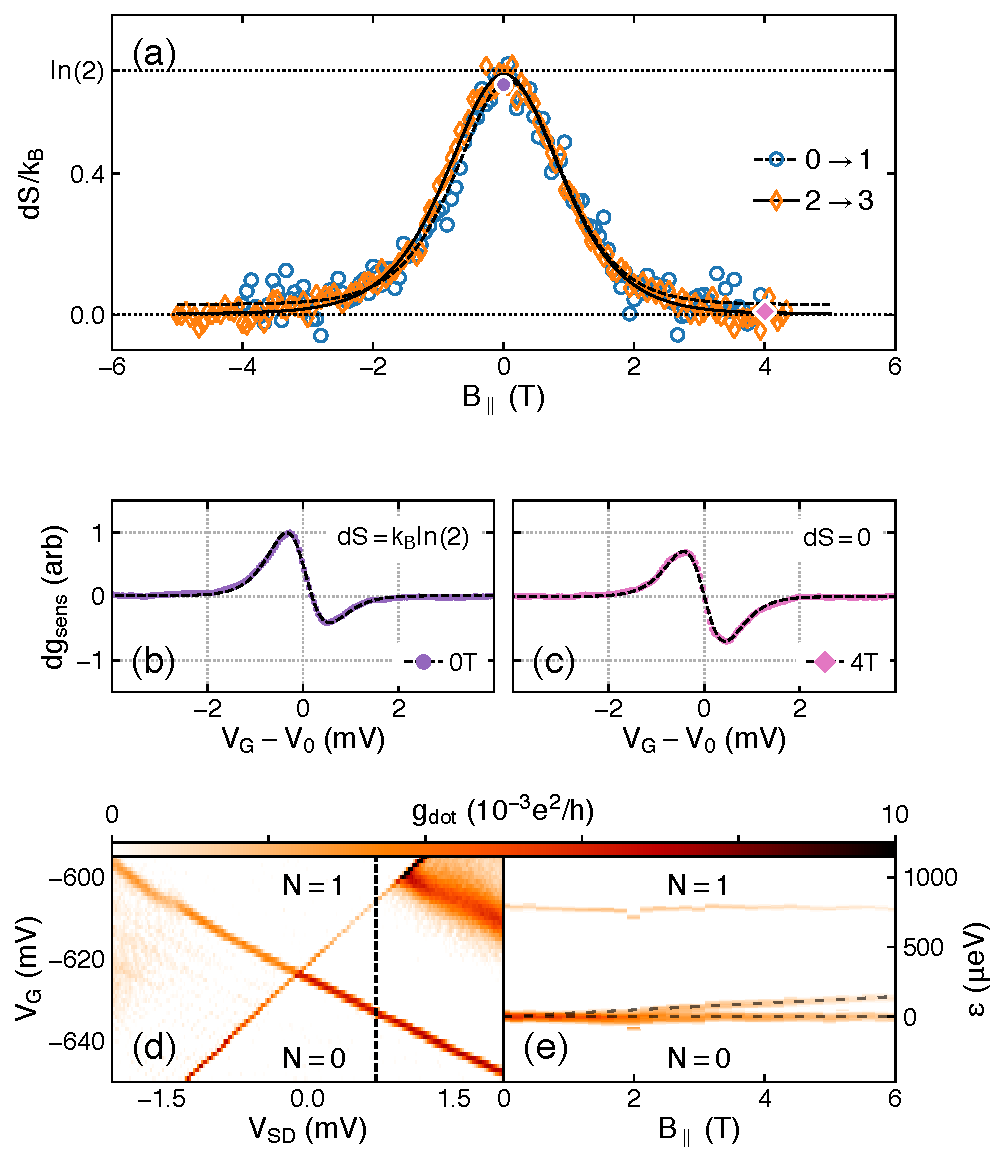
\includegraphics[width=1.0\columnwidth]{../figures/figure_3.pdf}
        \caption{\label{fig:fig3}(a) Transport data through the quantum dot showing the $N=0 \rightarrow 1$ transition. The first excited state, near $V_{SD} = $ \SI{1}{\milli\electronvolt}, is well-above all other energy scales in the measurement. Dashed line at $V_{SD}$ = \SI{700}{\micro\electronvolt} shows where data in (b) are taken. (b) Fixed bias transport data showing fits to the Zeeman splitting of the ground state energy from which $g = -0.44$ is extracted. (c) Change in entropy, determined from $dg_{sens}$ fits at varying parallel magnetic field. The $N=0 \rightarrow 1$ and $2 \rightarrow 3$ data are overlaid here to show the similar behavior of these states at low field. (d) and (e) show characteristic $dg_{sens}$ traces from which the data in (c) were extracted. These data points are show as large markers in (c)}
\end{figure}

Confirmation that the measured $dS$ derives from spin degeneracy can be seen in its evolution with in-plane magnetic field, $B_\parallel$. Figure \ref{fig:fig3}a [REMOVE PANELS AB] compares $dS(B_\parallel)$ for the 0-1 and 2-3 electron transitions.  The 2-electron ground state is a spin singlet, while the 3-electron ground state adds an additional unpaired electron, so both $dS_{0 \rightarrow 1}$ and $dS_{2 \rightarrow 3}$ correspond to transitions from total spin zero $(S_0=S_2=0)$ to total spin one-half, and one might expect identical field-dependent behaviors for $dS_{0\rightarrow 1}$ and $dS_{2\rightarrow 3}$ as long as $g \mu_{B} B_\parallel$ is less than the excited state energies.

The entropies of 1- and 3-electron states are suppressed when the Zeeman splitting lifts the spin degeneracy of the unpaired electron, following the Gibbs entropy for a two-level system:
%
\begin{align}
\label{eqn:gibbs}
        S &= k_B \sum_{i=\pm} p_{i}(B_\parallel, T) \ln{ p_{i}(B_\parallel,T) }
\end{align}
%
where $p_{\pm}(B_\parallel, T) = (1+ e^{\mp \frac{g\mu_B B_{\parallel}}{k_B T}})^{-1}$ are the probabilities for the system to be in $+/-$ (up/down) spin states at a given field and temperature. Fits to the lineshape in Eqn.~\ref{eqn:gibbs} are shown in Fig.~\ref{fig:fig3}a for both transitions, allowing for peak height, a vertical offset, and the ratio $g/T$ as free parameters.

The entropy measurement agrees quantitatively with the expected $k_{B} \ln{2}$ at $B_\parallel=0$, collapsing to zero at high field when spin degeneracy is broken.  Using a $T=T_{res}$ of 130 \SI{100}{\milli\kelvin} that is midway between the low ($T_{MC}$) and high ($T_{MC}+dT$) points of the temperature oscillation yields $g=0.43$ or $g=0.4$ for the $0\rightarrow 1$ and $2\rightarrow 3$ transitions respectively, consistent with the value $g=-0.44$ expected for GaAs and measured via bias spectroscopy in a separate measurement (Figs.~\ref{fig:fig3}bc).  At a qualitative level, the high-field crossover to a perfectly antisymmetric lineshape for $dg_{sens}(V_G)$ at the charge transition clearly indicates $\delta$ from Eqn.~\ref{eqn:dg} going to zero, corresponding to no entropy change between the two charge states (Figs.~\ref{fig:fig3}de). 

%%% figure 4 %%%
\begin{figure}
        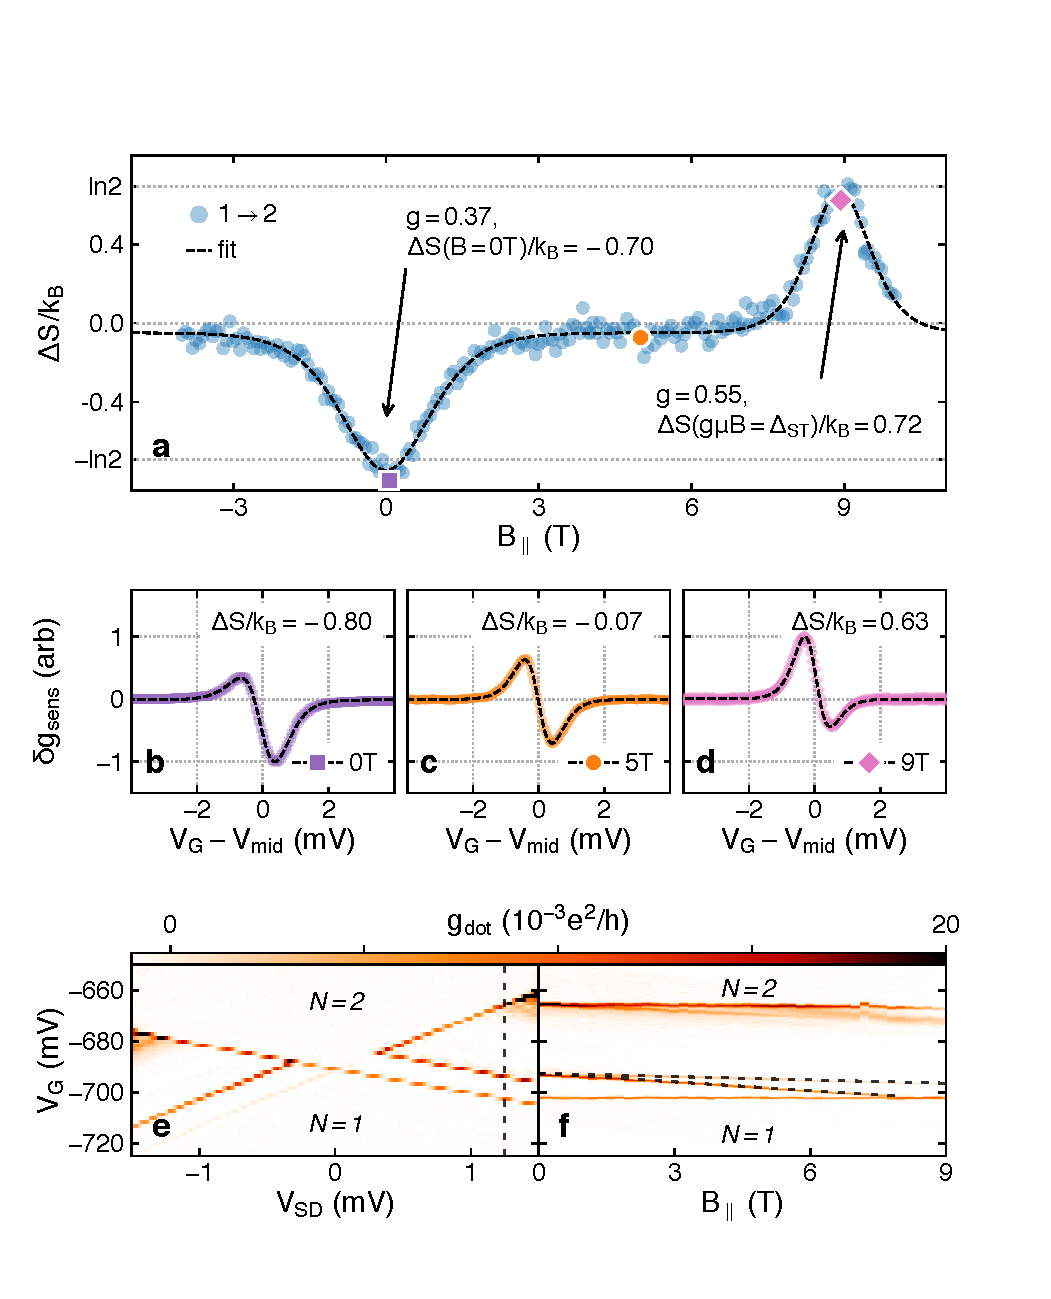
\includegraphics[width=1.0\columnwidth]{../figures/figure_4.pdf}
        \caption{\label{fig:fig4}(a) (a) Transport data through the quantum dot showing the $N=1 \rightarrow 2$ transition. Singlet-triplet splitting is roughly \SI{300}{\micro\electronvolt} and depends on applied field. Dashed line at $V_{SD}$ = \SI{1250}{\micro\electronvolt} shows where data in (b) are taken. (b) Fixed bias transport data in parallel field. The triplet level is split into $T_+$, $T_0$, and $T_{-}$ (not visible). At \SI[input-protect-tokens]{\sim 9}{\tesla} $T_+$ becomes degenerate with $S$. $g$ is determined using $T_0$ and $T_+$ fits. (c) Change in entropy, extracted from $dg_{sens}$ fits at varying parallel field. As the field goes from 0 to 10T, entropy of the 2-electron state goes from $0  \rightarrow \ln{2}$, while the entropy of the 1-electron state goes from $\ln{2} \rightarrow 0$. Fit to this behavior (dashed) is described in the text (d), (e), and (f) show characteristic $dg_{sens}$ traces from which the data in (c) were extracted. These data points are show as large markers in (c)}
\end{figure}

The entropy of the 0 and 2-electron states are both zero at low magnetic field, so $dS$ for the $1\rightarrow 2$ transition (Fig.~\ref{fig:fig4}a) can be understood as the inverse of Fig \ref{fig:fig3}a as long as $B_\parallel$ is less than around \SI{5}{\tesla}.  There, the 2-electron ground state remains in the spin singlet state with zero entropy while 1-electron ground state entropy goes from $k_B\ln{2}$ to zero due to Zeeman splitting. At higher field, the 1-electron ground state remains non-degenerate while the 2-electron ground state becomes two-fold degenerate where the singlet ($S$) and triplet ($T_+$) states cross. The singlet-triplet crossing is seen clearly around at \SI{9}{\tesla} in bias spectroscopy data for the $1\rightarrow 2$ transition (Fig.~\ref{fig:fig4}bc). 

The field-dependent entropy measurement for the 1-2 transition can again be fit using Eq.~\ref{eqn:gibbs}, with probabilities as before for the 1-electron states and $p_{S/T}(B_\parallel, T) = (1+ e^{\mp \frac{g\mu_B B_\parallel - \Delta_{ST}}{k_B T}})^{-1}$ for the 2-electron singlet-triplet states, where $\Delta_{ST}$ is the singlet-triplet splitting at zero field. The fit allows for an offset from $dS=0$, away from the degenerate points, to compensate for non-linearities in the charge sensor. From the fit we find the entropies at the two-fold degenerate points, $B=0$ and \SI{9}{\tesla}, are within 5\% of the expected values, $\mp k_B \ln{2}$. The extracted value of $g = 0.394$ from the low-field peak agrees well with the fit in Fig.~\ref{fig:fig3}a. At the high-field singlet-triplet degeneracy, $g = 0.586$ in the fit. This unexpected g-factor is explained by a shifting of the $T_{0}$ with magnetic field, as seen in Fig.~\ref{fig:fig4}f and previous work. The high quality of this Gibbs entropy fit confirms $dS$ can be related directly to a tunable degeneracy in the system.

%%% conclusion %%%
The results presented demonstrate a novel technique to measure the entropy of few-particle states in mesoscopic devices. The measurement was used to investigate the well-understood spin degeneracy of the few-electron ground states states in a GaAs quantum dot. The entropy signal is confirmed by tuning the entropy as a function of applied magnetic field. Future work may take advantage of this strategy to look for thermodyanmic signatures of non-trival electron and quasiparticle states, eliminating the uncertainty found in typical transport data.

\paragraph*{Methods} The device was built on a AlGaAs/GaAs heterostructure, hosting a 2D electron gas with density and mobility at \SI{300}{\milli\kelvin} (determined on a separate chip) of \SI{2.42e11}{\per\square\centi\metre} and \SI[per-mode=symbol]{2.56e6}{\square\centi\metre\per\volt\per\second}.   Mesas and NiAuGe ohmic contacts to the 2DEG were defined by standard photolithography techniques, then \SI{10}{\nano\metre} of $\mathrm{HfO_2}$ was deposited via atomic layer deposition to improve the gating stability to the device. Electron beam lithography followed by evaporation of \SI{20}{\nano\metre} of Ti/Au defined the fine gate structures, including the \SI{200}{\nano\metre} diameter quantum dots. The measurement was carried out in an dilution refrigerator with a base temperature of \SI{14}{\milli\kelvin}.

The conductance of the charge sensor was measured at a DC voltage bias of XXX uV, with the current read out directly or fed into a lockin amplifier.  The temperature of the reservoir could be raised above $T_MC$ (to $T_MC + dT$) using a current biased through the left (heater) QPC. A calibration for $dT$ in this mode, using DC current bias $\alpha$ as measured in Fig.~\ref{fig:fig2}b, can be seen in Fig.~\ref{fig:fig2}c. Applying AC current at $f_{Heat} =$ \SI{48.7}{\hertz} yields oscillations in $T_{res}$ at $2f_{heat}$; to leading order $dT_{res} \sim P \sim \cos(2*(2 \pi f_{heat})t)$. Variations in $g_{sens}$ with $dT$ are captured with a lockin amplifier measuring $g_{sens}$ oscillations at at the second harmonic of $f_{heat}$. 


%\acknowledgments
% Everyone I might acknowledge is currently an author. Consider moving someone here.

\bibliography{qdentropy}{}
\bibliographystyle{apsrev4-1}

\end{document}